\chapter{Prosody, prosodic prominence and focus}
\label{chapter_prosody}

Prosody denotes all aspects of the rhythmical and tonal organisation of spoken communication \citep{Calhoun2007}. Every utterance in every language has prosodic properties \citep{Grice2006}. Languages employ prosody to chunk the stream of speech and to single out certain elements in this stream, like words or syllables. Both mechanisms lend rhythmical and tonal structure to speech. The use of prosodic aspects to single out certain elements has been termed \emph{prosodic prominence}. Prosodic prominence is understood as a relative property as one element is made \emph{prominent} in comparison to other elements \citep{WagnerWatson2010}. Making a word or a syllable in a word more prominent often reflects the speaker's intention to highlight importance or newness of the word or referent denoted by that word in the discourse. Prominence and its relation to discourse play a major role in this work but the demarcating aspects and the marking of edges of prosodic constituents are also discussed to some extent in this chapter.

Among the physical parameters that have attracted most attention in the analysis of prosodic patterns are fundamental frequency (F0), intensity or amplitude, and duration \citep{Ladd2008, Grice2006}. Their perceptual counterparts are pitch, loudness and length. These parameters form a conglomerate of prosodic cues and neither of them is used exclusively for a certain function of prosody. They all play a role in both chunking as well as prominence. F0 movements on or close to a syllable as well as an increase in amplitude and duration can make this syllable stand out from neighbouring syllables. But an F0 movement and an increase in duration are also often used to mark the end of a phrase. In addition, spectral properties of vowels and consonants have been reported to be affected by prosody \citep{Cho2011, Gussenhoven2004}. For example, lending prosodic prominence to a syllable can affect the formant values of the vowel in that syllable. Vowels in more prominent positions tend to be less centralised compared to their counterparts in less prominent positions, revealing a more distinct articulation \citep{DeJong1995, Cho2005, Mücke2018}.

Decades of prosody research have emphasised that prosody has decomposable structure and that the relations of the elements within that structure are important to understand prosody \citep{Ladd2008, Arvaniti2011}. The next section sheds light on prosodic structure (Section \ref{sec:prosodic_structure}). Section \ref{sec:focus1} then takes to a first look at one of the most important functions of prosody in West-Germanic languages, namely the marking of \emph{focus}, and uses the knowledge of prosodic structure to explain the relation of focus and prosody. Section \ref{sec:prosody_catcont} investigates the categorical and continuous aspects of prosody and argues that prosody is characterised by both. In the light of this argumentation, Section \ref{sec:focus2} takes a second look at focus marking and shows that categorical and continuous aspects of prosody are involved in this function of prosody. Section \ref{sec:prosodic_strengthening} gives an overview on how prosody affects movements of supra-laryngeal articulation and points out a strong connection of prosodic structure and what has been described as segmental. Section \ref{sec:focus3} takes a third look at focus beyond tonal properties presenting evidence that prosodic strengthening plays an important role here as well. Section \ref{sec:summary_prosody} summarises the chapter.

\section{Prosodic structure}
\label{sec:prosodic_structure}

A very influential framework for the analysis of prosody is the auto-segmental model \citep{Pierrehumbert1980, Ladd2008}, henceforth: AM. This framework stresses the idea that prosodic structure is organised hierarchically and that the tune of an utterance, the \emph{intonation contour}, can be decomposed into smaller units (tones) that are to some extent independent of the words they are produced on. Different hierarchies of prosodic structure have been proposed in the literature \citep{NesporVogel1986, PierrehumbertBeckman1988, Hayes1989, Selkirk1996, ShattuckHufnagelTurk1996}. All proposals share the assumption that utterances can be decomposed into hierarchically organised constituents although they disagree as to the existence of some levels. Most researchers in the field agree upon a minimal structure that can be outlined as follows \citep{Grice2006}: An utterance consists of one or more intonational phrases which contain one or more smaller phrases. Here, an intermediate phrase is assumed as the level between the intonational phrase and the word. A constituent on the smallest level of phrasing contains one or more words, a word contains one or more feet, and a foot contains one or more syllables. This prosodic hierarchy is illustrated with an example in Figure \ref{fig:prosodic_hierarchy}.

\begin{figure}[h]
\begin{center}
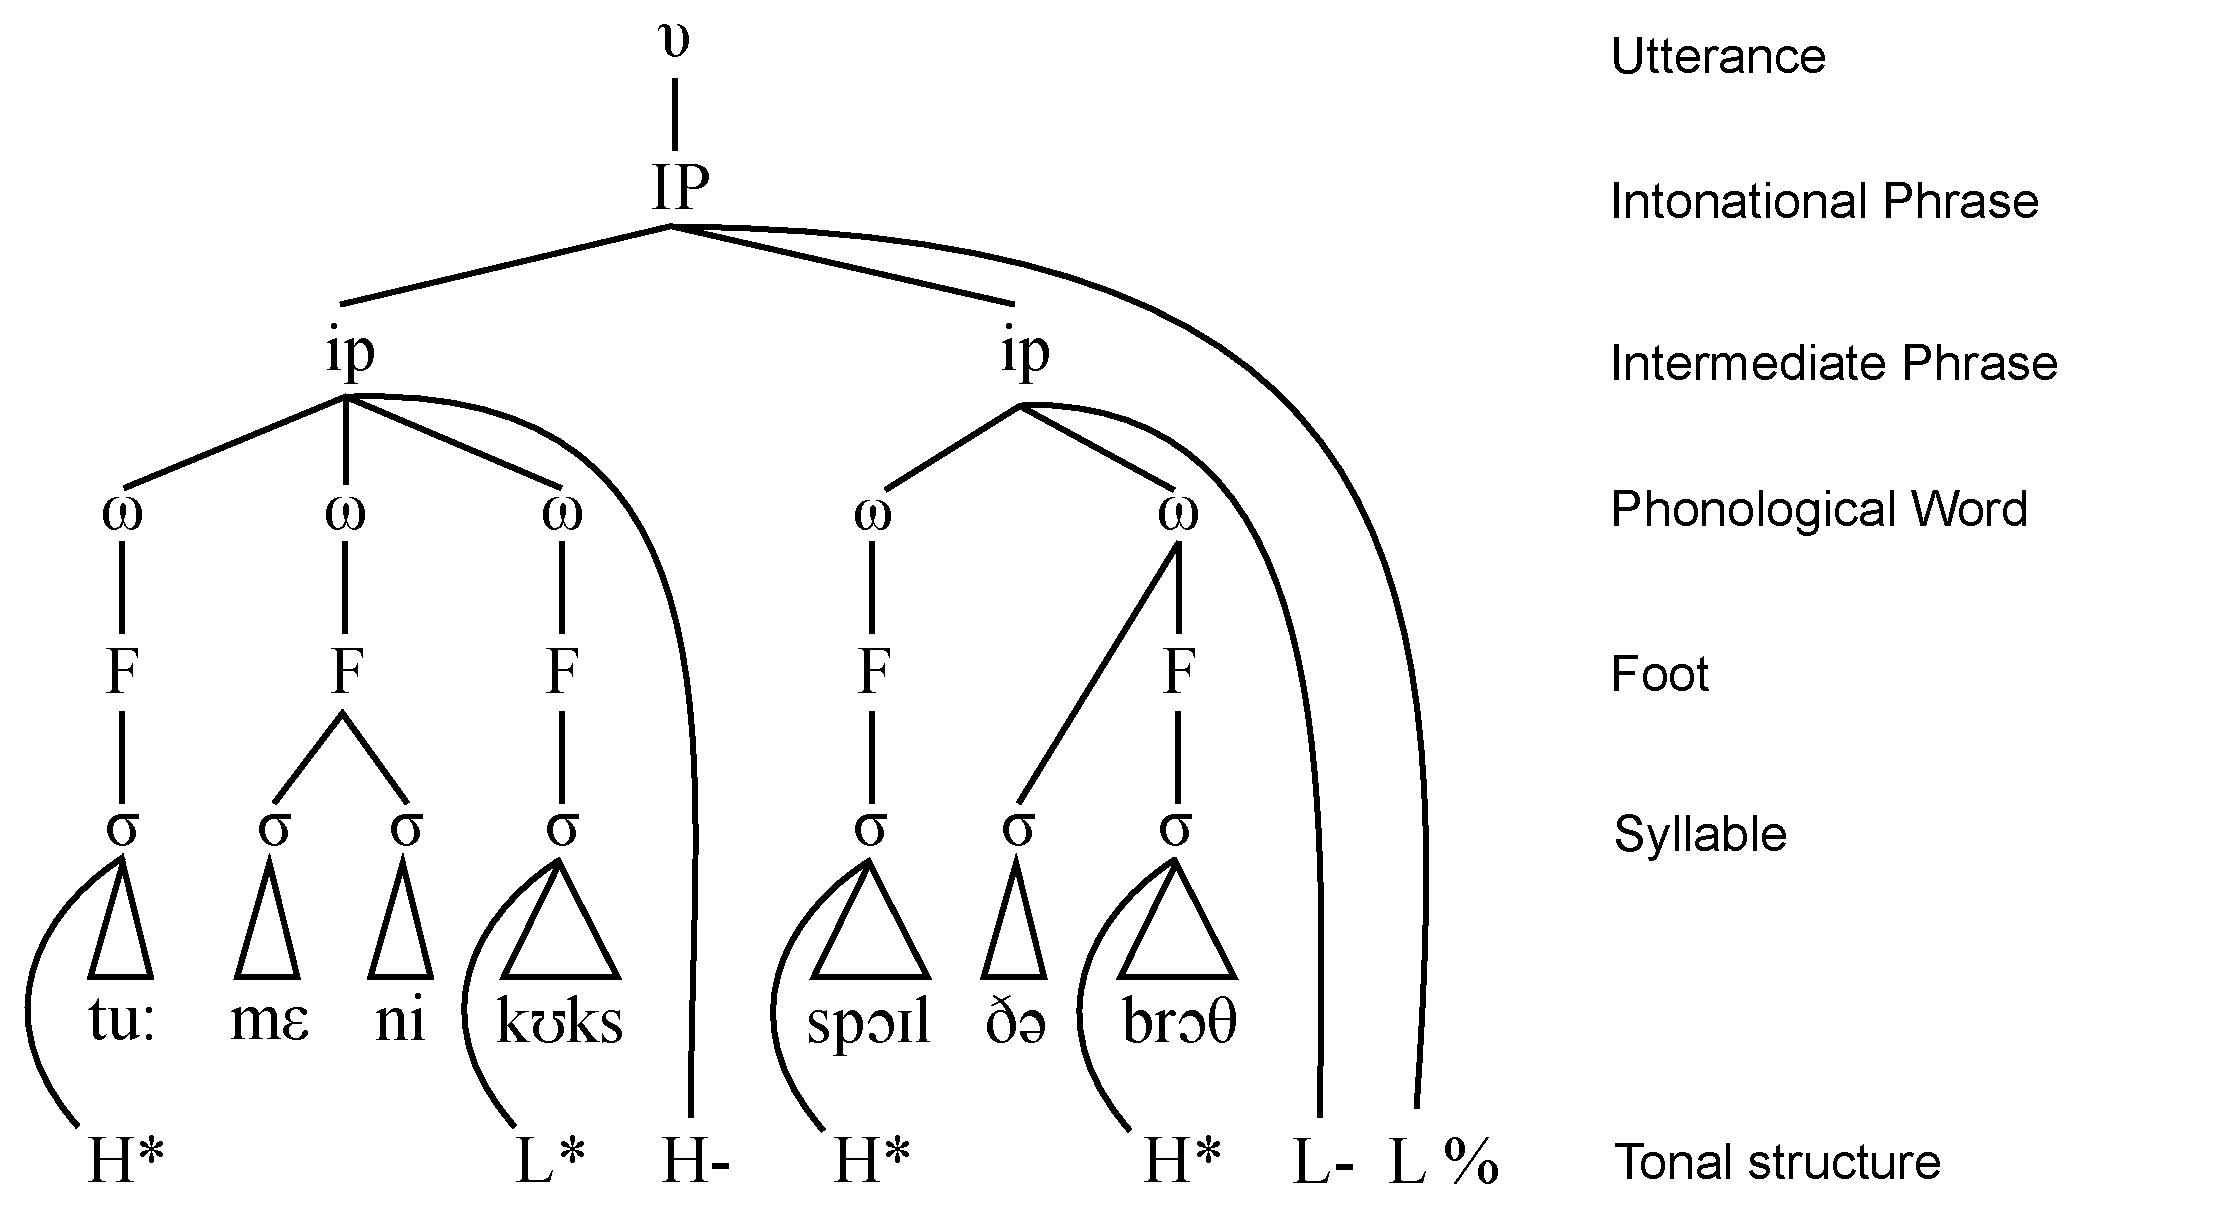
\includegraphics[width=\textwidth]{figures/ch4/prosodic_hierarchy.pdf}
\caption{Prosodic hierarchy for the sentence ``too many cooks spoil the broth" inspired by \citet{Grice2006} and \citet{Gussenhoven2004}.}
\label{fig:prosodic_hierarchy}
\end{center}
\end{figure}

An intonation contour in the AM framework is modelled as a string of high and low tones, H and L, that is associated with the constituents in the prosodic hierarchy. However, not every word or syllable in a phrase receives a tone. The string of tones is associated with the ``text", i.e. the syllables of a sentence, at certain points. Between the syllables where tones occur, the intonation contour is interpolated \citep{Ladd2008}. 

Tones can occur as \emph{pitch accents} or as \emph{boundary tones}. In many intonational languages -- like English, German and Dutch -- pitch accents are associated with primary stressed syllables in the prosodic hierarchy. The term pitch accent is used here in the sense of \emph{intonational pitch accent} as opposed to \emph{lexical pitch accent} \citep{Ladd2008}. Intermediate phrases can contain more than one pitch accent. Of all pitch accents, the last (fully fledged) pitch accent is called the \emph{nuclear pitch accent} \citep{Gussenhoven2004}. The placement of the nuclear pitch accent can be seen as a form of head-marking \citep{BeckmanEdwards1994, ShattuckHufnagelTurk1996} in which the most prominent syllable of the intermediate phrase is the head of this prosodic constituent and receives the nuclear pitch accent \citep{Grice2006}. A pitch accent is marked by the symbol * and can consist of one or two tones, e.g. H* or L+H*. In the latter case, i.e. in bitonal pitch accents, only one of the two tones receives the * and is called the \emph{starred tone}. The other tone occurs either before the starred tone, as in the case of a \emph{leading tone} (L+H*), or after the starred tone, as in the case of a \emph{trailing tone} (L*+H). 

Boundary tones occur on two levels. Both intermediate and intonation phrases have boundary tones. One convention (see for example GToBI: \citealp{GriceBaumann2002} and \citealp{GriceBaumannBenzmüller2005}) is to mark the boundary tone of an intermediate phrase with the symbol -, e.g. L-, and the boundary tone of an intonation phrase with the symbol \%, e.g. L\%. Since intermediate phrases are contained in intonation phrases, the end of an intonation phrase co-occurs with the end of the last intermediate phrase of the intonation phrase. The notation of the two boundary tones is T$_1$-T$_2$\%, where T stands for tone. If T$_1$ and T$_2$ are identical, only one of them is written, i.e. L-L\% is written as L-\%. 

The motivation of modelling an intonation contour as a string of tones rather than a holistic melodic unit comes from the observation that the intonation contour is not simply stretched or compressed when the number of syllables present in the sentence increases or decreases. Instead, the shape of the intonation contour is affected by the alignment of the tones relative to the syllables they are associated with \citep{Ladd2008, Arvaniti2011}. The example in Figure \ref{fig:me_ballgown} illustrates this point: It shows a schematised version of a contour prominently discussed in the literature by \citet{HirschbergWard1985}, \citet{HirschbergWard1992}, \citet{Arvaniti2011}, \citet{Ladd2008} and many others. The contour is used to express incredulity towards a suggestion made by the interlocutor. On the left, the realisation on the mono-syllabic phrase ``Me?!” is shown. The intonation contour rises, falls and rises again. This contour could be described as a holistic rise-fall-rise pattern \citep{Ladd2008}. On the right, the figure shows two options of adjusting the contour to be realised on a longer phrase. In the upper plot, the holistic rise-fall-rise shape of the contour is simply stretched to span the longer phrase. However, this is not the way the contour is realised on longer phrases \citep{Arvaniti2011}. The actual realisation of the contour is represented by the schematisation in the lower plot and demonstrates that the contour is best described as a composition of separate tonal events. The phrase starts low, the rise-fall movement is timed roughly with the syllable ``ball” and not stretched over several syllables. The final rise of the contour is realised at the very end of the utterance, most probably on the last syllable of ``designer”. There is a low stretch of F0 in between these two events. An analysis within the AM framework decomposes this contour into a pitch accent and a rising boundary tone at the end of the phrase. The pitch accent is associated with the most prominent syllable in the phrase, ``ball”, and gets aligned with it in time. The boundary tone is associated with the phrase and marks the edge of this phrase. As a consequence, its rising tonal movement is realised towards the end of the phrase. In between these two tonal events, the low stretch of F0 represents an interpolation that can be extremely short as in the case of ``Me?!" or longer depending on the number of syllables between the accent and the edge \citep{Ladd2008} . 

\begin{figure}[h]
\begin{center}
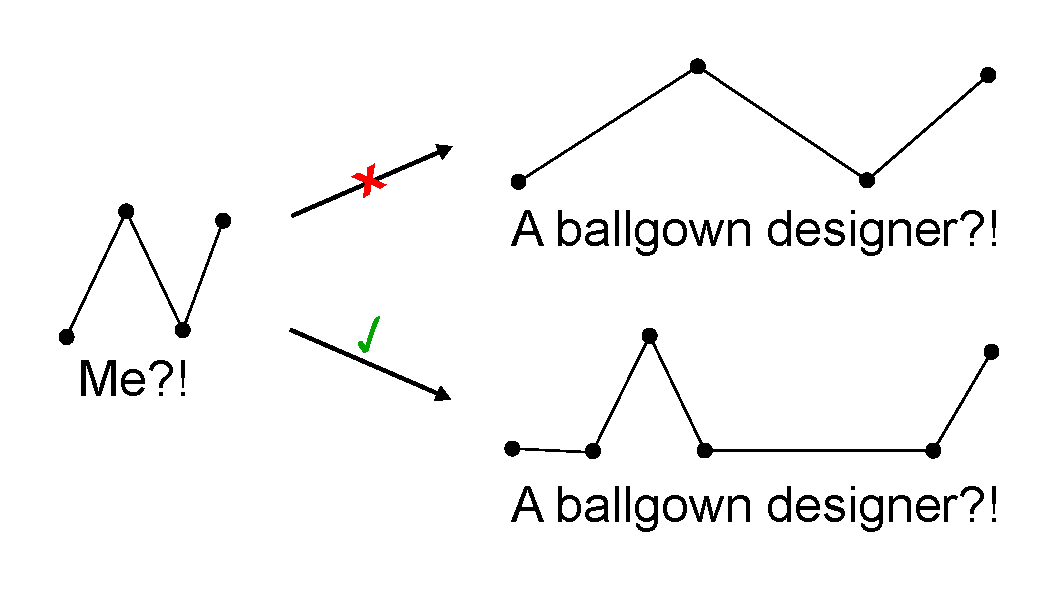
\includegraphics[width=8cm]{figures/ch4/me_ballgown.pdf}
\caption[Schematic illustration of an intonation contour expressing incredulity.]{Schematic illustration of an intonation contour expressing incredulity \citep{HirschbergWard1992}. The right side shows two hypothetical options how the short version can be enlarged for longer sentences.}
\label{fig:me_ballgown}
\end{center}
\end{figure}

A possible analysis in the AM tradition \citep[as in ToBI:][]{BeckmanHirschbergShattuckHufnagel2005} would describe the contour as L*+H L-H\%\footnote{The fact that the phrase starts low is accounted for with a default boundary tone that is described as mid or low in the speaker's range and, being the default, is omitted from the transcription.} with the L of the boundary tone spreading ``leftwards" to the end of the pitch accent to create a low stretch on the non-prominent syllables after the pitch accent. Depending on the inventory of pitch accents and boundary tones (e.g. presence of leading and/or trailing tones), models in the AM framework can differ in their description of the same contour. The common assumption, however, is that the contour can be decomposed into tonal events and that such a description is better able to capture generalisations on intonational structure and meaning than a holistic approach.  

\section{A first look at prosodic focus marking}
\label{sec:focus1}

In West-Germanic languages, like German, Dutch and English, the placement of a pitch accent is used as a means to package the information conveyed by a sentence. In these languages, prosody plays a role in signalling which parts of the utterance are in \emph{focus}, and which are in the \emph{background} \citep{Lambrecht1994}. This structure, the \emph{focus structure} of the sentence, manifests the speaker's beliefs about how the information of the sentence fits the knowledge of the listener \citep{Vallduvi1992}. The focus constituent includes the information that the speaker believes to be significant, the background constituent contains information that is less relevant \citep{Gussenhoven2004}. Often, the focus constituent contains new information while the background contains given information, but this is not always the case. In the above-mentioned languages, the focussed part usually receives the nuclear pitch accent. The background constituent usually does not receive the nuclear pitch accent and is often completely unaccented, in particular when the background part follows the focus part (also known as \emph{post-focal deaccentuation}).

Consider the example in \ref{ex:broad_focus}. The answer contains only new information \citep{Ladd1980, Gussenhoven2004}, nothing is given by the question, everything is in focus. This condition is often called \emph{broad focus} \citep{Ladd1980}. In this case, the nuclear pitch accent is usually placed on the last noun, ``Jana”. Even though ``Jana" receives the nuclear pitch accent, this does not mean that it is the only word in focus. The mechanism that assigns the nuclear pitch accent within the focussed constituent is called \emph{focus projection} \citep{Büring2003, Ladd2008}. The word that receives the nuclear pitch accent functions as the \emph{focus exponent} for the larger focus domain \citep{Ladd2008}. 

\begin{equation}
\begin{tabular}{ll}
Q: & 	Was gibt’s Neues?\\
&	What’s up?\\
A: &	[Melanie will Jana treffen.]$_F$\\
&	[Melanie wants to meet Jana.]$_F$
\end{tabular}
\label{ex:broad_focus}
\end{equation}

In example \ref{ex:narrow_focus}, the question triggers a different focus structure in the answer. The new information is contained in the word ``Jana” only. The focus structure of this example is called \emph{narrow focus} \citep{Ladd1980, Gussenhoven2004}. As in the example before, the pitch accent is placed on the word ``Jana".

\begin{equation}
\begin{tabular}{ll}
Q: & 	Wen will Melanie treffen?\\
&	Who does Melanie want to meet?\\
A: &	Melanie will [Jana]$_F$ treffen.\\
&	Melanie wants to meet [Jana.]$_F$
\end{tabular}
\label{ex:narrow_focus}
\end{equation}

A special case of narrow focus is illustrated in example \ref{ex:contrastive_focus}. Again, all information except for ``Jana” is given by the question. In addition, ``Jana” serves as a direct alternative to the referent ``Peter” given in the question. The nuclear pitch accent is again placed on the word ``Jana”. This focus structure is often labelled \emph{contrastive focus} or \emph{corrective focus} \citep{Gussenhoven2004}.

\begin{equation}
\begin{tabular}{ll}
Q: & 	Will Melanie Peter treffen?\\
&	Does Melanie want to meet Peter?\\
A: &	Melanie will [Jana]$_F$ treffen.\\
&	Melanie wants to meet [Jana.]$_F$
\end{tabular}
\label{ex:contrastive_focus}
\end{equation}

So far, the pitch accent location did not change in the examples as a function of the focus structure of the sentence. Either the last noun was the only focussed element (narrow and contrastive focus) or it served as the focus exponent for a larger focus domain (broad focus). Example \ref{ex:background} demonstrates what happens if the focus is earlier in the sentence. The example in fact shows a case of contrastive focus. This time, however, the focussed element is ``Melanie”. As a consequence, the nuclear pitch accent is placed on ``Melanie” and the part of the utterance after this word, ``will Jana treffen”, is in the background. This part is deaccented and characterised by a low stretch of F0, lower amplitudes and shorter durations.

\begin{equation}
\begin{tabular}{ll}
Q: & 	Will Paul Jana treffen?\\
&	Does Paul want to meet Jana?\\
A: &	[Melanie]$_F$ will Jana treffen.\\
&	[Melanie]$_F$ wants to meet Jana.
\end{tabular}
\label{ex:background}
\end{equation}

Moving the nuclear pitch accent to a different word as a means of packaging the information is a very well described phenomenon in intonation languages like English, German and Dutch. Other intonation languages like Spanish and Italian do not use the manipulation of the nuclear pitch accent location to mark focus structure or do so only to a limited extent \citep{Ladd2008}. Languages that use nuclear pitch accent location to mark focus have been called \emph{plastic} languages, those that do not have been called \emph{non-plastic} languages \citep{Vallduvi1991}.

Although manipulating the location of the nuclear pitch accent is a very well documented and salient feature of focus marking, this is not to say that focus structures with the nuclear pitch accent in the same place are identical with regard to their prosodic realisation. Later in this chapter, evidence for fine-grained strategies of prosodic focus marking will be discussed. The second part of this book presents a large data pool supporting and extending this evidence. It will become clear that both categorical and continuous modulations are used in the differentiation of focus structures. Therefore, before turning to this central issue, it is useful to take a closer look at what is known about categorical and continuous characteristics of prosody. 

\section{The nature of prosody: categorical and continuous}
\label{sec:prosody_catcont}

The outlined view of intonation in the AM framework is characterised by the assumption of discrete events in tonal structure. The last two sections sketched the motivation for this perspective. First, as illustrated by the example of the ``incredulity contour" (see Figure \ref{fig:me_ballgown}), it is plausible to analyse intonation contours as composites. Some units that form these composites are associated with strong syllables while others are associated with phrase constituents. Hence, the wide-spread approach of AM intonation analysis posits that categoriality is a major feature of the structure of intonation contours: Tones can belong to the categories pitch accent or boundary tone. 

Second, the examples of focus realisation in German (\ref{ex:broad_focus}, \ref{ex:narrow_focus}, \ref{ex:contrastive_focus}, and \ref{ex:background}) have added another important aspect of categorical patterning in the analysis of intonation. It is a discrete choice which syllable a pitch accent (in this case the nuclear pitch accent) is associated with. The pitch accent is either associated with syllable A or B (or C or...). Moreover, different types of pitch accents exist in the AM analysis. This means that while there is a possible syntagmatic contrast between a syllable that receives a pitch accent and one that does not, there are also possible paradigmatic contrasts between pitch accent types. A pitch accent can be of type A or B (or C or...), or in AM terms: H* or L* or H+L* (or L+H* or...). Models within the tradition of AM draw pitch accents from a closed inventory and consider these pitch accent types as phonologically distinct. Analogously, boundary tones are also given as a closed set of distinctive types.

The identification of categoriality in the structure of intonation forms the basis of the ``intonational phonology" \citep{Ladd2008} put forward by scholars in the AM framework. However, it is not restricted to this framework and has antecedents in other models. For instance, intonation analysis in the tradition of the \emph{British School} \citep{OConnorArnold1973} identifies categorical distinctions on multiple levels. Pitch accented syllables are distinguished from other categories of prominence (secondary stress, tertiary stress, unstressed). Moreover, intonation contours are decomposed into parts like head, nucleus and tail. With regard to the \emph{nuclear tone}, consisting of the nucleus and the tail, the British School has attempted to identify distinct tunes that evoke differences in meaning, like ``high fall" or ``low rise" \citep{Cruttenden1997}. In the \emph{IPO} model of intonation \citep{tHartCollierCohen1990} -- named after the Institute of Perception Research, in Dutch: Instituut voor Perceptie Onderzoek -- similar to the analysis of the AM framework, a distinction is made between pitch movements associated with boundaries and pitch movements associated with prominences. Tonal patterns are described in terms of a composition of ``categorically distinct entities" \citep[14]{Ladd2008}, e.g. ``Type A Fall" or ``Type 1 Rise". 

To conclude, the assumption of the categorical, phonological status of intonation contours or building blocks of contours plays a significant role in various aspects of the description of intonation. Experimental approaches have been developed to assess the notion of categoriality in intonation empirically. For example, \citet{PierrehumbertSteele1989} manipulated the timing of the accentual peak of a rise-fall-rise contour on the sentence ``Only a millionaire" from relatively early to relatively late with 13 intermediate steps.\footnote{The ``relatively early peak" L+H* in this experiment should not be confused with the general notion of an early peak accent that is usually transcribed as H+L* or H+!H*.} The resulting 15 stimuli represented a continuum between two contours that can be described as L*+H L-H\% and L+H* L-H\% with the pitch accent associated with the syllable ``mil". Apart from the alignment of the accentual peak with the accented syllable, the contour was unaltered. The subjects participating in the study were asked to listen to a stimulus and imitate it. The authors' prediction was the following: If the nature of the difference between the two pitch accent types is categorical, the subjects should not be able to reproduce the continuum exactly. The data should instead cluster around two alignment patterns, one representing L*+H and the other one representing L+H*. If, on the contrary, alignment is used as continuous dimension in the intonation of American English, the subjects should be able to reproduce the continuum faithfully.

The result showed that almost all participants produced patterns that more or less clustered around two points on the continuum of peak alignment, yielding bimodal distributions for almost all speakers. Interestingly, although the results of the study suggest that peak alignment is used in a categorical fashion rather than continuously, two interesting observations can be made. First, the relative sizes of the two modes of the bimodal distributions differ across speakers, indicating that the continuum of stimuli is divided differently by individual speakers. Most speakers categorise a larger portion of the continuum as L+H* but there is also one speaker that divides the continuum into two approximately equal parts. Second, the modes of the alignment distributions of individual speakers are located differently in time. Both observations show that categories like L*+H and L+H* are not invariantly linked to patterns of phonetic implementation. 

Results pointing towards a categorical use of tonal alignment were also obtained by \citet{DImperioHouse1997}, investigating the intonation of narrow focus statements and yes/no questions in Neapolitan Italian. In this variety of Italian, both narrow focus statements and yes/no questions are characterised by a rising nuclear pitch accent followed by low boundary tone. The pitch accent of the narrow focus statement is analysed as H* while the pitch accent of the yes/no question is analysed as L+H*. According to \citet{DImperioHouse1997}, this difference is at least partially expressed with respect to timing of tonal events: The accentual peak of the H* is reported to be reached earlier than the peak of L+H*. The stimuli of this study comprise a five step continuum from relatively early (H*) to relatively late peak (L+H*). One set of stimuli was synthetically produced on the basis of the natural production of a statement and another set was produced on the basis of a question.

In contrast to \citet{PierrehumbertSteele1989}, a different experimental design was employed by \citet{DImperioHouse1997} to elicit the subject's responses. Participants were asked to listen to the continuum and categorise the stimuli they just heard as a question or a statement. The results showed that subjects categorise the earlier peak (H*) as a narrow focus statement and the later peak (L+H*) as a yes/no question as expected. Around the mid-point of the continuum, the proportions of ratings for both categories are around 50\% and the variability in the responses is high -- a response pattern expected for categorical oppositions. It should be noted, however, that these effects are clearest for stimuli that were resynthesised from a natural production of a statement. Additional evidence for the role of temporal alignment in the categorisation of pitch accent types comes from \citet{DilleyHeffner2013} for American English as well as \citet{Kohler1987} for German.

\citet{GussenhovenRietveld2000} provided support for categoriality of pitch accents in Dutch. The authors investigated the difference between a ``high rise" and ``low rise" question contour. In the former contour, the nuclear accented syllable is mid-pitched. In the latter contour, the nuclear accented syllable is low. Both contours are characterised by a rise from the accented syllable to the end of the phrase. In terms of an AM analysis, the contours could be described as H* H-H\% and L* H-H\% \citep{Gussenhoven2004}. The experimental paradigm of \citet{GussenhovenRietveld2000} is based on the observation that speakers expand the pitch range when speaking in an emphatic or surprised fashion. Accordingly, subjects were presented with artificial contours in which the height of both the accentual target (L* or H*) and the boundary tone target (H-H\%) were manipulated. 

The results are in line with the prediction that what is analysed as a phonological low tone (L) behaves differently from what is analysed as a phonological high tone (H) when the pitch range is expanded. A L* accent is perceived as ``more surprised" when realised lower whereas a H* accent is perceived as ``more surprised" when realised higher. These results suggest that it is plausible to describe the accent as belonging to two different categories. At the same time, they reveal that intonational meaning, in this case ``surprise", is carried by continuous variation as well. In addition, the results of \citet{GussenhovenRietveld2000} show that the implementation of categories is subject to contextual variation and not invariant.

The experiment of \citet{GussenhovenRietveld2000} was based on the assumption that pitch range constitutes a parameter continuously varied by speakers. \citet{LaddMorton1997} questioned the purely continuous nature of pitch range as a parameter of intonation. The authors sought empirical evidence for the existence of \emph{normal} and \emph{emphatic} peak pitch accents as two distinct categories in British English. This distinction is assumed to be (at least partially) expressed by pitch range with the emphatic accent having a larger pitch range than the normal accent. Since in this study phrases with only one accent are used, it remains open whether pitch range is interpreted ``globally" on the level of the phrase or ``locally" on the level of the accent. Regardless of which interpretation is to be favoured, one can speak of a difference in \emph{pitch excursion}, manifested phonetically in the relation between the F0 target of the peak on the accented syllable and the F0 target of the low boundary following.

The findings of \citet{LaddMorton1997} on the categorical use of pitch excursion remain inconclusive and thereby provide an interesting example of the study of categoriality and continuity in intonation. The methodology of the study included both rating on a scale as well as forced choice tasks. In a first perception experiment -- which was designed to be a norming study to test the usefulness of the speaker's voice and the manipulation strategies -- the authors randomly played stimuli from a continuum of pitch excursions to 35 subjects. This continuum consisted of resynthesised contours based on natural utterances produced in either a ``normal" or an ``emphatic" fashion. The pitch excursion on the continuum was increased in steps of 6 Hz. Two instructions to elicit the participants' answers were used. In the first instruction, the participants were asked to rate the degree of emphasis on a ten-point scale. In the second instruction, two different interpretations were presented, ``a neutral statement" and ``a contradiction or correction". The participants were asked to rate on a ten-point scale how likely the interpretations were. The results show that stimuli manipulated from an emphatic natural basis were interpreted as more emphatic, a finding that indicates that emphasis is expressed by more than just pitch excursion. Apart from this effect, both sets of stimuli evoked similar responses: The larger the pitch excursion, the more ratings towards an ``emphatic" interpretation. This trend showed no clear discontinuities that would be expected for a categorical difference.

In a second experiment, \citet{LaddMorton1997} used a subset of the stimuli from the first experiment and employed a classic categorical perception paradigm consisting of two forced choice tasks, an \emph{identification task} and a \emph{discrimination task}. In the identification task, subjects listened to a stimulus from the continuum and judged whether the sentence described an ``everyday occurrence" or an ``unusual experience". In the discrimination task, subjects listened to pairs of stimuli in quick succession and were asked to choose whether they were the same or different. The stimuli of a pair were either neighbours on the manipulated continuum and thus differed by 6 Hz or were identical. 

The responses of the identification task provided the classic S-shaped curve expected for the presence of two categories. The curve showed that in the region between 138 and 156 Hz, the responses abruptly become more variable and tend towards 50\%, i.e. subjects were less certain about the interpretation of the stimuli. This result alone does, however, not suffice to attest the existence of two distinct categories of normal and emphatic. It has to be kept in mind that the subjects had only two options to choose from. To provide clearer evidence for categoriality, the discriminability of stimuli must increase in the region of the putative category boundary. Remember that the pairs of different stimuli played in the discrimination task consisted of neighbours on the continuum differing by 6 Hz. Subjects should perform better at discriminating stimuli belonging to different categories compared to stimuli belonging to the same category. In fact, in the study of \citet{LaddMorton1997}, subjects were better at discriminating stimuli pairs at the putative category boundary. However, the discrimination rate was rather low even in this region. In addition, the discrimination rates at the ends of the acoustic continuum, i.e. within the assumed categories, were also larger than zero.

While the findings of \citet{LaddMorton1997} do not support categorical perception of normal and emphatic pitch accents in a strict sense, they suggest that the continuum was not completely linearly perceived. These observations reflect the fact that pitch excursion may be used in a categorical and continuous way at the same time. For example, transcription systems in the AM tradition acknowledge that H* and L+H* accents are, among other parameters, distinguished in terms of in the magnitude of the rise towards the starred tone H* \citep{GriceBaumann2002}. The rise is described as steeper and higher for L+H* compared to H*. Thus, in this case, local pitch excursion is one phonetic parameter to differentiate phonological categories. At the same time, this parameter is used in a continuous fashion. The continuous use can be the result of global or local pitch range expansions to signal emotional affection or surprisal (as in the case of Gussenhoven and Rietveld's experiment) or to make a distinction between different accent types clearer. The latter case might be classified as a kind of intonational hyperarticulation in the sense of Lindblom's (\citeyear{Lindblom1990}) Hyper- and Hypo-Articulation theory (H\&H theory).

Striking similarities are found for the phonetic parameter of temporal alignment of an accentual peak. At the beginning of this section, evidence has been presented for the existence of a categorical implementation of this parameter. However, it is also known that later alignment of an accentual peak may be used in addition to increased pitch excursion -- or even as a substitute for increased pitch excursion -- to increase prominence in intonation languages like German and English \citep{Gussenhoven2004, LaddMorton1997}. A possible explanation might be that higher pitch excursions take longer to be executed. Therefore, higher peaks have a potential physiological correlate of delay, a mechanism that speakers may have ``tacit knowledge" of \citep[90]{Gussenhoven2004}. Regardless of the validity of this explanation, the observation is interesting for two reasons. First, it shows that alignment is used in a continuous manner as well. Second, while the symbiosis of pitch excursion and alignment is conceptualised as a phonetic effect, it is also manifested in the description of intonational categories: In addition to a difference in the magnitude of the rise towards the high accentual target (as already mentioned above), the distinction of H* and L+H* in German ToBI is based on a difference in alignment. A later peak alignment is attributed to the L+H* accent in comparison to the H* accent in this model.

Essentially, these observations suggest a deep intertwining of the use of prosodic parameters to establish phonological categories on the one hand and their direct, continuous (or: phonetic) use on the other. The next section will present evidence on the realisation of focus types that provides support for the idea of an interrelation of phonetic and phonological aspects of intonation developed in the present section.

\section{A closer look at prosodic focus marking}
\label{sec:focus2}

Earlier in this chapter, the use of nuclear pitch accent placement in West-Germanic languages to mark focus structure was introduced. It was noted that the placement of the nuclear accent might not change as a function of focus structure in some cases. In the examples, the nuclear accent remained on the word ``Jana", the last noun, regardless of whether the focus structure was broad focus, narrow focus or contrastive focus. The literature nevertheless discusses prosodic ways of  differentiation between these focus types.

For American English, \citet[296]{PierrehumbertHirschberg1990} state that the L+H* pitch accent ``evokes a salient scale". It is described to mark contrastive focus as opposed to the H* accent that -- combined with a low boundary tone -- contributes to a ``neutral declarative intonation" \citep[290]{PierrehumbertHirschberg1990}. \citet{WatsonTanenhausGunlogson2008} add supporting evidence for the interpretation of L+H* as marking contrastive focus in an eye-tracking study. They note, however, that the uses of L+H* and H* seem to overlap.

For German, \citet{Baumannetal2007} found that the proportion of downstepped H* accents, i.e. !H*, is highest in broad focus. The number of upstepped H* accents, \^{}H*, is highest in contrastive focus. Plain H* accents are predominantly found in narrow focus. While the distributions are overlapping, in line with the perceptual findings of \citet{WatsonTanenhausGunlogson2008}, these results by \citet{Baumannetal2007} indicate that different pitch accent types are used to signal different focus types. Crucially, the predominantly used accent types are characterised by increasing acoustic salience from broad focus to narrow focus, and from narrow focus to contrastive focus \citep[see][]{BaumannRöhr2015}. The results are supported by data presented in \citet{BaumannGriceSteindamm2006} that show fewer downstepped accents in narrow compared to broad focus, and fewer downstepped accents in contrastive compared to narrow focus. 

Contrary to these findings, \citet[63]{Fery1993} reported no difference between broad and narrow focus. The divergence of the results might be attributed to the fact that the speech material of this study is different from the sentences used in above-mentioned studies by \citet{Baumannetal2007} and \citet{BaumannGriceSteindamm2006} (and the examples given earlier in the present chapter). Another explanation might be sought in the fact already mentioned several times in this discussion: The distributions of pitch accent types used for different functions are overlapping. Hence, there does not seem to be a one-to-one mapping of pitch accent type to focus type.

\citet{Griceetal2017} investigated the categorical and continuous aspects of intonational patterns used to mark focus structures by 5 German speakers (data also reported on in \citealp{MückeGrice2014}). The speech material used was very similar to the examples \ref{ex:broad_focus}, \ref{ex:narrow_focus}, and \ref{ex:contrastive_focus}. Their analysis comprised both symbolic annotations as well as measurements of continuous, phonetic parameters. Figures \ref{fig:grice_etal_2017_PA_types} and \ref{fig:grice_etal_2017_PA_types_speakers} give a first insight into their data by showing the GToBI nuclear pitch accent distributions based on consensus annotations by two annotators. Figure \ref{fig:grice_etal_2017_PA_types} gives the distributions for all speakers together and confirms the finding outlined above, namely that there is not a one-to-one mapping of pitch accent type to focus type but that there are tendencies: Most falling accents, H+!H*, can be found in broad focus, most accents with a steep rise, L+H*, can be found in contrastive focus. Narrow focus seems to be positioned in between with a rather high number of H* accents but also a considerable number of L+H* and even H+!H* accents. Figure \ref{fig:grice_etal_2017_PA_types_speakers} presents the distributions for each speaker separately. While for some speakers (F1 and F2) the overall tendency of Figure \ref{fig:grice_etal_2017_PA_types} can be observed at least for the differentiation of broad focus and contrastive focus, for other speakers (F3 and M2), a different picture is obtained. These speakers use one pitch accent category predominantly for all three focus types. In the case of speaker F3, it is H*; in the case of speaker M2, it is L+H*. Speaker M1 seems to use a mixed strategy between the two groups. This speaker differentiates broad and narrow focus by using different pitch accent types, but shows almost exclusively L+H* accents in both narrow and contrastive focus.

\begin{figure}[htp]
\begin{center}
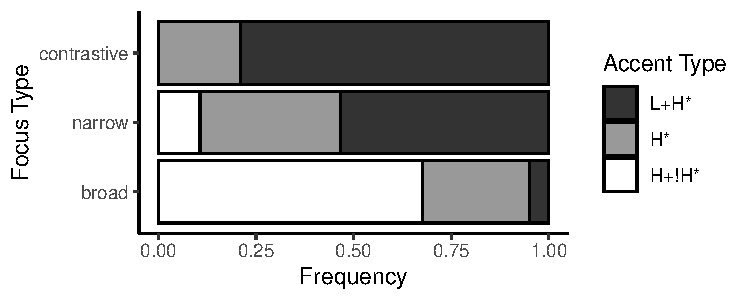
\includegraphics[width=11cm]{figures/ch4/Grice_etal_PA_Types.pdf}
\caption{Nuclear pitch accent type distributions in the data set of \citet{Griceetal2017}.}
\label{fig:grice_etal_2017_PA_types}
\end{center}
\end{figure}

\begin{figure}[htp]
\begin{center}
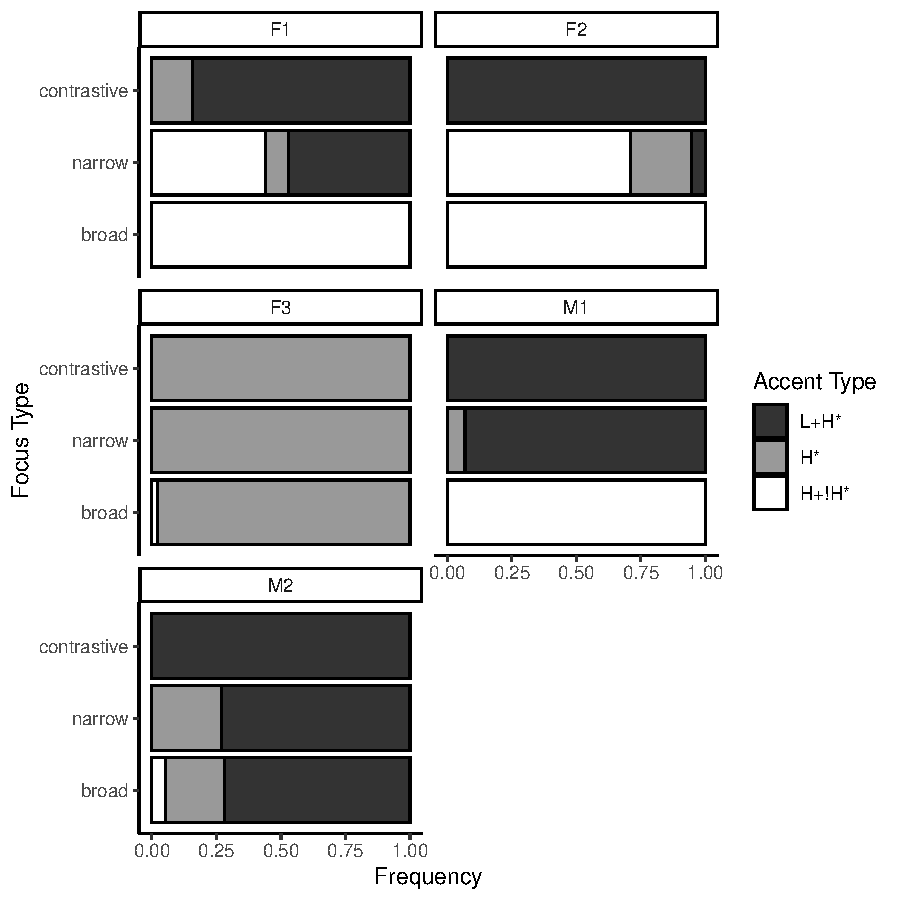
\includegraphics[width=\textwidth]{figures/ch4/Grice_etal_PA_Types_Speakers.pdf}
\caption{Nuclear pitch accent type distributions in the data set of \citet{Griceetal2017} for each speaker separately.}
\label{fig:grice_etal_2017_PA_types_speakers}
\end{center}
\end{figure}

The data of \citet{Griceetal2017} was used in a perception test by \citet{CangemiKrügerGrice2015} and \citet{Krüger2009}. Their results showed that all five speakers were ``able to convey their pragmatic intentions to listeners in a comparable way" \citep[91]{Griceetal2017}. This conclusion is rather surprising with regard to the different pitch accent distributions and considering that some speakers do not differentiate the focus types clearly in terms of their pitch accent choice. Motivated by the discrepancy of pitch accent choice and scores in perception testing, the analysis by \citet{Griceetal2017} went beyond the description of intonational patterns using pitch accent types and investigated various continuous parameters. Interestingly, their results reveal that the speakers' strategies are not as disparate as the pitch accent distributions suggest. Figure \ref{fig:grice_etal_2017_alignment} shows the mean alignment values of the peak of the nuclear pitch accent in relation to the onset of the accented syllable.\footnote{The original paper uses the alignment relative to the accented vowel onset which yields comparable results. The current figure is based on the openly available data set which contains both alignment relative to the onset of the accented syllable (that has a CV structure) as well as alignment relative to the onset of the accented vowel.} Note that the peak does not have to belong to the starred tone (as in the case of H* and L+H*). In H+!H* accents, the peak is part of the leading tone (H+). The alignment data reveal the same pattern for all five speakers: Broad focus has the earliest peak alignment, contrastive focus has the latest peak alignment, narrow focus is in between the two extremes: broad < narrow < contrastive. For the speakers that showed pitch accent type differentiation (F1 and F2, partly M1), the alignment modification ``crosses" category boundaries of pitch accent types. H+!H* accents in broad focus, for example, contribute negative alignment values as opposed to clearly positive values for L+H* accents in contrastive focus. For the other speakers (F3 and M2, partly M1), the alignment is modified within the boundaries of a single category. In other words, the parameter alignment is used in both continuous, ``phonetic" and categorical, ``phonological" ways but the general trend of modification, or the direction of modification, is invariant across speakers.

\begin{figure}[htp]
\begin{center}
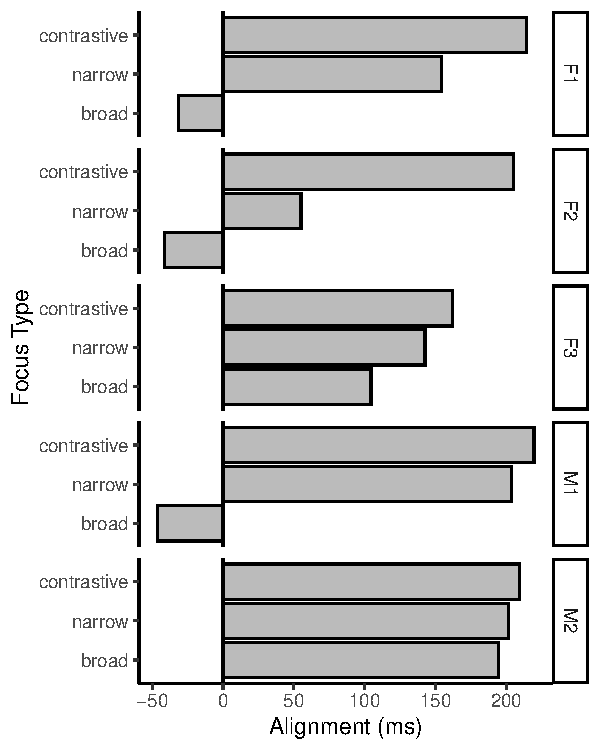
\includegraphics[width=9cm]{figures/ch4/Grice_etal_Alignment.pdf}
\caption{Mean alignment of the peak relative to the onset of the accented syllable in the data set of \citet{Griceetal2017} for each speaker separately.}
\label{fig:grice_etal_2017_alignment}
\end{center}
\end{figure}

In addition to the alignment of the peak, \citet{Griceetal2017} measured the \emph{tonal onglide} \citep{RitterGrice2015}, a parameter that plays an important role throughout the following parts of this work. The tonal onglide is a means to assess the F0 movement towards the main tonal target of the accent -- in AM terms, the starred tone. In the version that \citet{Griceetal2017} employed, the tonal onglide is quantified as the difference in semitones between the starred tone target and a fixed point 30 ms before the onset of the accented syllable. If the accent is falling, the resulting tonal onglide is negative, if the accent is rising, the tonal onglide is positive. This means that the tonal onglide gives an indication of the movement of the accent (falling vs. rising) but also of the magnitude of this movement. It is comparable to the measure of alignment by answering the question whether the accent is an early peak accent like H+!H* or a mid to late peak accent like H* or L+H*. But it also assesses pitch excursion continuously, for example by quantifying the magnitude of the rise in accents like L+H*.

In Figure \ref{fig:grice_etal_2017_onglide}, the results of the tonal onglide measure from \citet{Griceetal2017} are shown. The picture obtained here is comparable to the results for the peak alignment -- it is even clearer in some cases. All speakers manipulate the tonal onglide in the same direction. Broad focus has the smallest tonal onglide values, contrastive focus has the largest, narrow falls in between: broad < narrow < contrastive. As in the case of alignment, some speakers cross clear category boundaries. For example, the negative tonal onglide values of F1, F2 and M1 in broad focus are an indication of accents of the falling type H+!H* whereas the positive onglide values in contrastive focus result from the frequent use of the rising accent type L+H*. Crucially however, a speaker like F3 that exhibits only H* accents in the categorical analysis of Figure \ref{fig:grice_etal_2017_PA_types_speakers} differentiates the focus types in terms of onglide values. The same is true for speaker M2 and the difference between narrow and contrastive focus in speaker M1.

\begin{figure}[htp]
\begin{center}
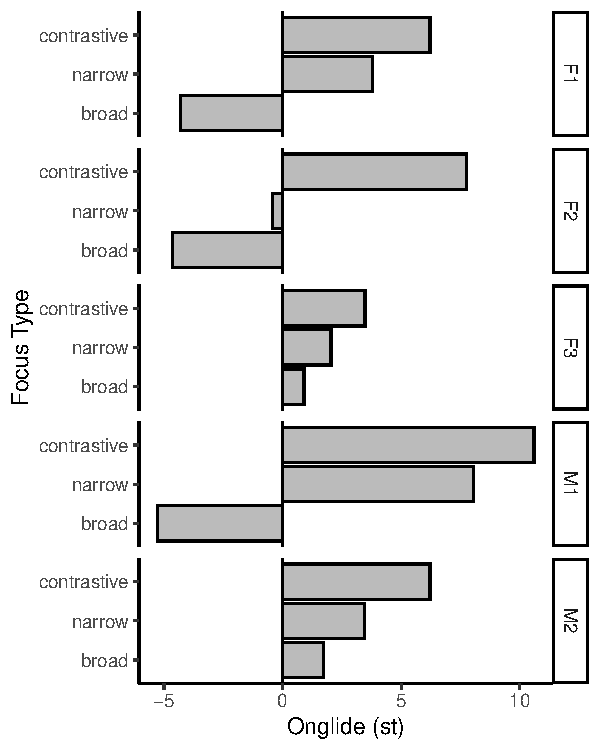
\includegraphics[width=9cm]{figures/ch4/Grice_etal_Onglide.pdf}
\caption{Mean tonal onglide values in the data set of \citet{Griceetal2017} for each speaker separately.}
\label{fig:grice_etal_2017_onglide}
\end{center}
\end{figure}

Both alignment and tonal onglide give a deeper insight into strategies of focus marking. What appears to be disparate strategies in a symbolic account is shown to be very similar when looking at the continuous parameters in addition to the symbolic transcription. Moreover, the results suggest that there might be no clear boundary between a categorical and a continuous use of intonation to mark focus types. Rather, speakers seem to integrate the two uses with a clear mutual trend. As the perception results of \citet{CangemiKrügerGrice2015} and \citet{Krüger2009} show, listeners are able to use the information encoded in the speech signal, regardless of whether the differences are in terms of what is described as pitch accent categories or more subtle and subsymbolic variation. This finding resonates well with the remark of \citet[88]{Ladd2014} discussed in Chapter \ref{chapter_pandp} that categorical and continuous variation commonly go hand in hand and very often ``are likely to interact and reinforce one another".

\section{Prosodic strengthening}
\label{sec:prosodic_strengthening}

So far, this chapter has concentrated on tonal aspects of prosody. A large body of research shows, however, that many other aspects play an important role as well. One important aspect is that the articulation of consonants and vowels -- also often called \emph{supra-laryngeal} articulation as opposed to \emph{laryngeal} articulation that produces tone -- is affected by prosodic structure \citep{Mücke2018}. More specifically, it has been shown that some positions in the prosodic hierarchy are characterised by ``stronger" articulation to increase syntagmatic and paradigmatic contrasts. Often, articulatory gestures are expanded in the spatio-temporal domains \citep{Cho2011}. This phenomenon, termed \emph{prosodic strengthening} \citep{Cho2006}, can be observed as a result of marking the boundaries of prosodic units, like an intonational phrase, but also as a concomitant of accentuation, e.g. in syllables with the nuclear pitch accent. This section attempts to give an overview on parts of this research that are most relevant to the topic of the present work, and will thus focus on prominence-induced strengthening.

Speakers have multiple possibilities to express prominence in the speech signal. As has been discussed extensively in this chapter, the placement of a (nuclear) pitch accent is a very important prosodic feature -- perhaps the principal feature in this regard. A pitch accent is characterised by a pitch movement around the syllable that bears it. However, as introduced above, amplitude, and duration \citep{Ladd2008, Grice2006} as well as spectral properties of vowels in the accented syllable \citep{Cho2011, Gussenhoven2004} have been identified as important prosodic parameters. Under the influence of accent, amplitude and duration are increased, and the spectral properties of vowels and consonant are modified \citep{Cho2011}. The source of all these modulations can be found in various modifications of supra-laryngeal articulatory patterns during the production of syllables under accent \citep{Mücke2018, Cho2005, DeJong1995, BeckmanEdwardsFletcher1992, DeJongBeckmanEdwards1993, HarringtonFletcherBeckman2000, ChoMcQueen2005, MückeGrice2014}.

The research literature describes different strategies of supra-laryngeal articulatory marking of accent in the case of vowels. One strategy that has been discussed is \emph{sonority expansion} \citep{BeckmanEdwardsFletcher1992}. Sonority expansion enhances the sonority of the vowel to strengthen the syntagmatic contrasts between accented and unaccented syllables. This strategy reflects the speaker's intention to produce louder and more sonorous
syllables by opening the mouth wider as a more open oral cavity allows for a greater radiation of acoustic energy from the mouth.

Another strategy is referred to as \emph{localised hyperarticulation} \citep{DeJong1995}. Based on the H\&H theory developed by \citet{Lindblom1990}, it follows the observation that prosodic prominence is expressed by a more extreme articulation of the tongue body in vowel productions. This strategy is often connected to the enhancement of paradigmatic features such as the place feature for a specific vowel. The tongue body position becomes lower in hyperarticulated low vowels such as /a/, while it is more fronted in front vowels such as /i/ and more retracted in back vowels such as /ʊ/ \citep{DeJongBeckmanEdwards1993, HarringtonFletcherBeckman2000, ChoMcQueen2005}.

Sonority expansion and hyperarticulation are highly overlapping strategies in low vowels like /a/. Opening the mouth wider and lowering the jaw and the tongue both achieve a higher sonority as well as a hyperarticulated, more distinct lower vowel. In other vowels, for example high vowels, the strategies may compete. Opening the mouth wider and lowering the jaw counteracts the raising of the tongue that is necessary to hyperarticulate a high vowel, i.e. to make it higher. There is, however, evidence that it is possible to combine the two strategies in the coordination of different articulatory subsystems that are used independently to some degree. Speakers may use the lingual system to hyperarticulate the place feature in high vowels such as /i/ and /ʊ/, while the mandibular and the labial system contribute to sonority expansion by increasing the degree of lip opening \citep{HarringtonFletcherBeckman2000}.

Regardless of the strategy pursued by the speaker, modifications found in the articulatory movements can be described in terms of variation in the parameters of the gestural model of Articulatory phonology that is based on the critically damped harmonic oscillator. Figure \ref{fig:cho_2006} presents an overview following \citet{Cho2006} on the possible parameter changes. In (a) a change in stiffness is shown. In the exposition of the harmonic oscillator model in Chapter \ref{chapter_ds}, stiffness corresponds to the parameter $k$. With higher stiffness values, the target is reached earlier, the velocity of the movement is increased.\footnote{While the parameter stiffness relates to the temporal organisation of the gesture only in this definition, it is defined in different ways in the literature. \citet[465]{MunhallOstryParush1985} define stiffness as a tempo-spatial parameter such that  ``higher stiffness corresponds to shorter duration [of] movements and greater peak velocity/movement amplitude ratios".} In (b) a change in the intergestural timing is shown. If a gesture is activated earlier, it can truncate a preceding gesture before this gesture reaches its target. Remember that temporal overlap was used in modelling assimilation in Chapter \ref{chapter_pandp}. There, overlap took place on different tiers, i.e. in different tract variables. The result was that one gesture was hidden. If overlap takes place in the same tract variable, truncation is the outcome. In (c) a change in the target is illustrated. The target corresponds to the parameter $x_0$ in the harmonic oscillator model. With a larger target to be reached in the same time, the velocity of the movement increases as well. In (d) a simultaneous change in target and stiffness is shown, resulting in a scaling (shrinking or enlargement) of the gesture.

\begin{figure}[htp]
\begin{center}
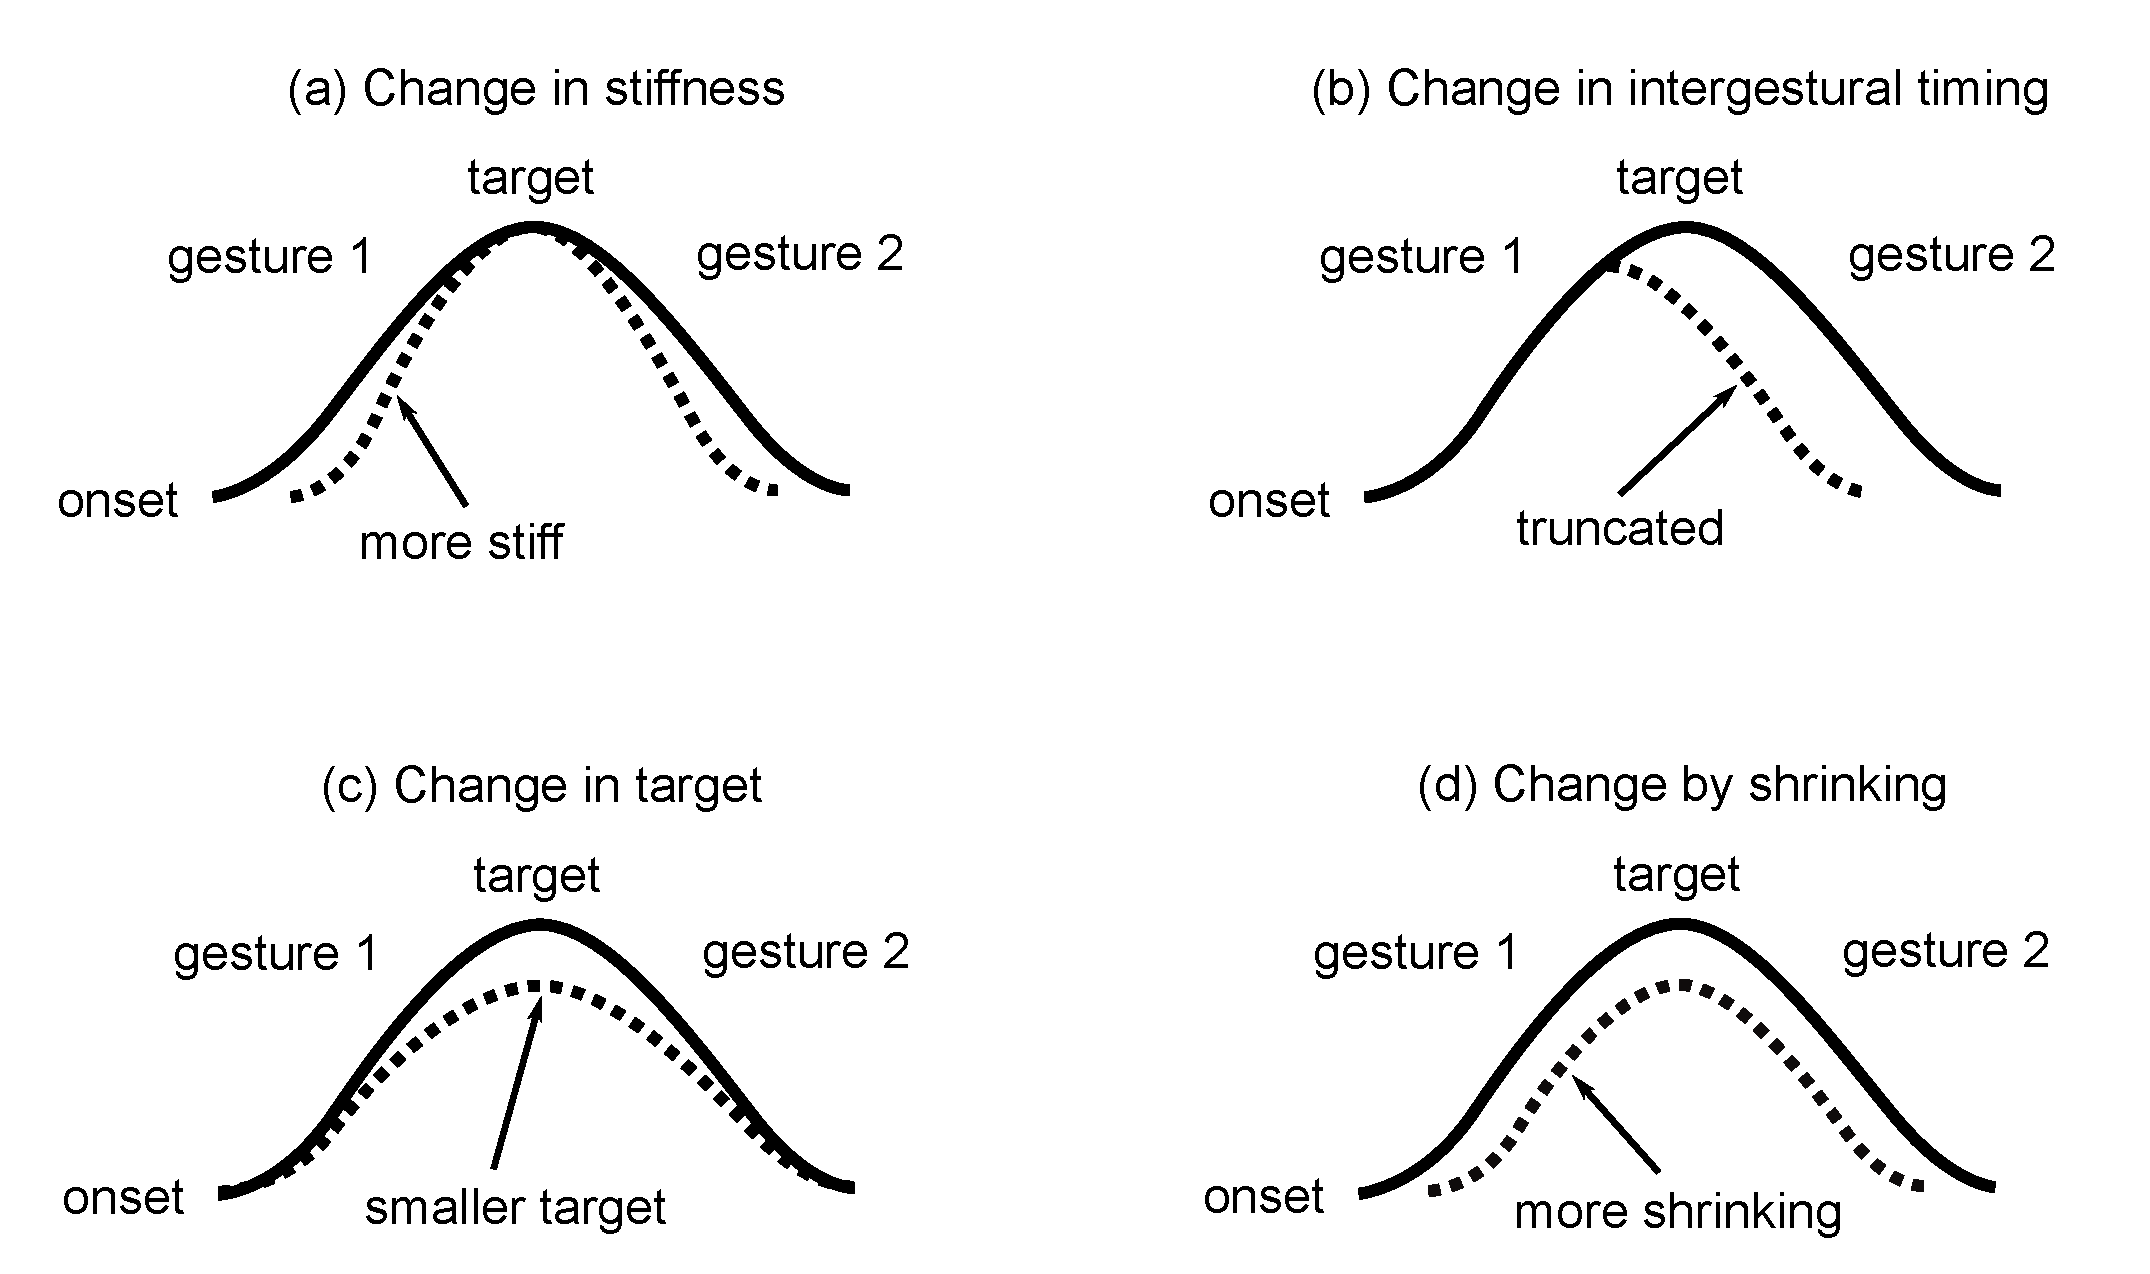
\includegraphics[width=\textwidth]{figures/ch4/cho_modifications.pdf}
\caption{Modifications of articulatory gestures induced by prominence following \citet{Cho2006}.}
\label{fig:cho_2006}
\end{center}
\end{figure}

The effect of prosodic structure on articulation, resulting in the modification of gestures as shown above, can be modelled using \emph{prosodic gestures}. Prosodic gestures are conceptualised as special gestures without any constriction. They exert control on the individual gestures responsible for the constrictions to produce vowels and consonants. This approach was developed to account for the fact that gestures are executed slower and overlap less in time at prosodic boundaries \citep{Byrd2000, ChoKeating2001, Fougeron2001, Tabain2003, Cho2006, KrivokapicByrd2012}. The proposal of \citet{Byrdetal2000} and \citet{ByrdSaltzman2003} is a prosodic gesture, called $\pi$-gesture, that modulates the intergestural timing at prosodic boundaries by modifying the stiffness of the constriction gestures co-activated with it. The extent to which the ``local speaking rate", i.e. the stiffness of gestures, is affected depends on the strength of the $\pi$-gesture \citep[13]{Byrd2000}. The activation level of the $\pi$-gesture is defined by the rank of the constituent in the prosodic strength.

While the $\pi$-gesture models what happens at prosodic boundaries, the $\mu$-gesture has been developed to account for the modifications of articulatory gestures under prominence. Initially proposed to account for the effect of stress \citep{Saltzmanetal2008}, it comes in two different versions. The $\mu_T$-gesture is slows down the constriction gestures in the interval of activation like the $\pi$-gesture \citep{Krivokapic2014}. The $\mu_S$-gesture modulates the spatial properties of the constriction gestures. Although developed for stress, $\mu_S$-gestures can be applied to the level of accent as well.

\section{Prosodic focus marking beyond tone}
\label{sec:focus3}

With regard to focus structure, the results of \citet{MückeGrice2014} give interesting insights into how speakers use the modification of supra-laryngeal articulation. The study used the same data set as \citet{Griceetal2017} with the three focus types broad, narrow and contrastive focus. In addition, the data set contains material of a fourth condition in which the target word is in the background, i.e. out-of-focus. This condition corresponds to example \ref{ex:background}. Remember that in this condition the target word does not receive an accent. 

All target words in this data set are disyllabic with stress on the first syllable that is either /bi:/, /ba:/ or /bo:/. The authors measured the duration and the displacement of the opening gesture of the lips from the maximal constriction of the lips for the bilabial stop to the maximal opening for the vowel.

The data of \citet{MückeGrice2014} show that there is a gradual increase in the duration and displacement of the opening gesture from background to contrastive focus with intermediate values for broad and narrow focus, see Figure \ref{fig:muecke_grice_2014}. Interestingly, there does not seem to be a big step between background and broad focus, i.e. between unaccented and accented. In fact, \citet{MückeGrice2014} find a statistically significant effect between the two conditions for only one speaker (F1). In contrast to this finding, the modifications between broad focus and contrastive focus seem to be much larger. 

\begin{figure}[htp]
\begin{center}
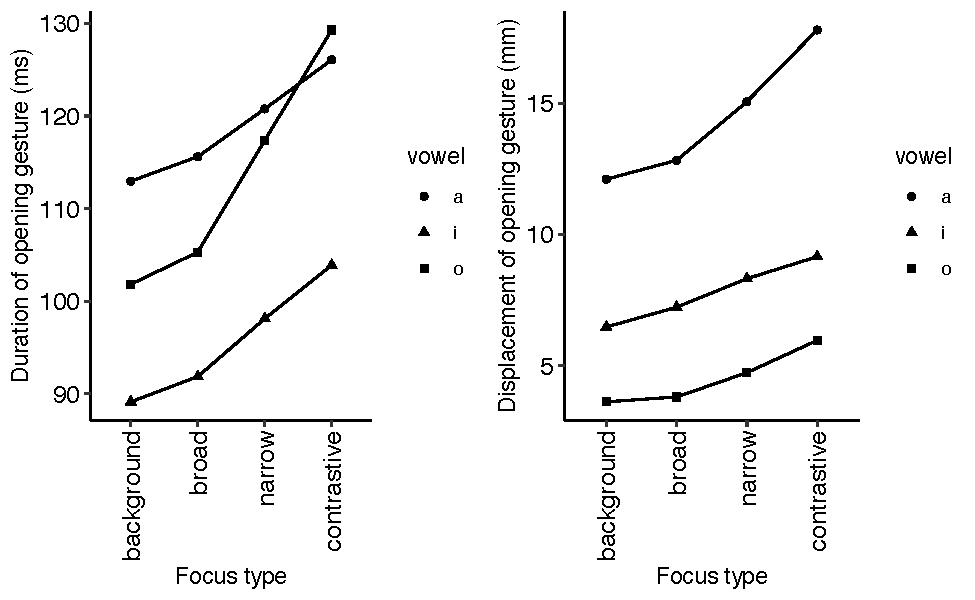
\includegraphics[width=\textwidth]{figures/ch4/muecke_grice_2014.pdf}
\caption{Mean duration and displacement of the vocalic opening gesture of the lips in the stressed syllable from the study of \citet{MückeGrice2014}.}
\label{fig:muecke_grice_2014}
\end{center}
\end{figure}

These data suggest that accented words do not necessarily have to be articulated differently from unaccented words (at least in the investigated articulatory dimensions). In addition, modifications of the supra-laryngeal articulation are used to encode focus structures that have the nuclear pitch accent in the same place (broad, narrow and contrastive focus all have the nuclear pitch accent on the target word). The latter result aligns well with the findings of \citet{Griceetal2017} that show tendencies to enhance prosodic prominence by choice of pitch accent type and the phonetic parameters of the pitch accent (alignment, onglide) from broad to narrow focus and from narrow to contrastive focus. It indicates that placing a nuclear pitch accent on a word is not the only important mechanism and that prominence is marked beyond accentuation. In addition to the categorical property of accentuation, continuous modulations play a significant role in the supra-laryngeal as well as the laryngeal system. These observations provide strong support for a view that acknowledges the importance of categoriality and continuity in prosody.

\section{Summary}
\label{sec:summary_prosody}

This chapter has been a whirlwind exploration of important concepts of prosody, prosodic structure and prosodic prominence. It has reviewed arguments for why it is reasonable to consider prosody as shaped by both categorical and continuous traits. The prosodic expression of focus was considered from different perspectives as focus is one of the most important functions of prosody in West-Germanic intonation languages. In addition, studies dealing with the prosodic marking of focus have revealed interesting results concerning the categorical and continuous aspects of prosody and their integration. The data presented in the following chapters of this book will also concentrate on focus and take the studies of \citet{MückeGrice2014} and \citet{Griceetal2017} as a basis for the experimental design, attempting to advance their conclusions by providing a formal modelling account.



